\documentclass[12pt,a4paper]{report}

\usepackage{graphics}
%\usepackage{fullpage,epsf,graphicx, amstext,url} 
%\usepackage{epsf}
\usepackage{graphicx}
\usepackage{amstext}
\usepackage{url}
\usepackage{amssymb}
\usepackage{graphicx}
%\graphicspath{ {/home/george/Desktop/Tex_Dissertation/images} }
%
% head.sty is no longer needed
%
%\usepackage{head,fullpage,epsf,graphicx, amstext,url} 

\def\BibTeX{{\rm B\kern-.05em{\sc i\kern-.025em b}\kern-.08em
    T\kern-.1667em\lower.7ex\hbox{E}\kern-.125emX}}

\begin{document}

\thispagestyle{empty}

%                       This is a basic LaTeX Template
%                       for the MSc Dissertation report
%
\parindent=10pt          %  Switch off indent of paragraphs 
\parskip=5pt            %  Put 5pt between each paragraph  
%
%                       This section generates a title page
%                       Edit only the sections indicated to put
%                       in the project title, and submission date
%

\vspace*{0.1\textheight}

\begin{center}
        \huge{\bfseries Calculation of the Supersymmetric top quark mass at CLIC}\\
\end{center}

\bigskip

\begin{center}
        \large{Georgios Billis}\\      % Replace with your name
        \bigskip
        \large{August 18, 2017}        % Submission Date
\end{center}

%%% If necessary, reduce the number 0.4 below so the University Crest
%%% and the words below it fit on the page.
%%% Don't let the crest and the wording below it flow onto the next page!
\vspace*{0.35\textheight}

\begin{center}
        
\includegraphics[width=35mm]{crest.pdf}
\end{center}

\medskip

\begin{center}

%%%
%%% Change Theoretical to Mathematical if appropriate
%%%
\large{
  MSc in Theoretical Physics\\[0.8ex]
  The University of Edinburgh\\[0.8ex]
  2017
}

\end{center}

\newpage


\pagenumbering{roman}

\begin{abstract}
In this project I calculate the mass of the Supersymmetric top quark in CLIC experiment at $\sqrt{s}$ = 3 TeV in $e^{-}$ $e^{+}$ collisions. I assume the following decay for the top squark $\tilde{q} \rightarrow q$ $\chi_{0}$, 
and I focus on the fully hadronic channel of decay i.e $\tilde{q} \rightarrow q$ $\chi_{0} \rightarrow$ $W b \tilde{\chi}_{1}^{0}$ .
The mass was found  to be  $m_{\tilde{t}}$ = 861 $\pm$ 19 GeV using the Boosted Descision 
Trees Multivariate Analysis and $m_{\tilde{t}}$ = 812 $\pm$ 20 GeV using the Gradient Boosted Descision  Trees Multivariate Analysis. 
\end{abstract}

\pagenumbering{roman}


\textbf{Declaration}


\newpage

\tableofcontents
\listoftables
\listoffigures

\begin{titlepage}
\vspace*{2in}
% an acknowledgements section is completely optional but if you decide
% not to include it you should still include an empty {titlepage}
% environment as this initialises things like section and page numbering.
\section*{Acknowledgements}

Put your acknowledgements here. Thanking your supervisor for his/her
help is standard practice, but you don't have to do this\ldots

This template is is modification of the one for the MSc in High
Performance Computing, which is apparently descended from a template
developed by Prof Charles Duncan for MSc students in Meteorology. His
acknowledgement follows:

\emph{This template has been produced with help from many former
  students who have shown different ways of doing things. Please make
  suggestions for further improvements.}

Some parts of this template were lifted unashamedly from the Edinburgh
MPhys project report guide, with little or no modification. I have no
idea who wrote the first version of that\ldots

You don't have to use \LaTeX\ for your dissertation. You can use
Microsoft Word or Apple Pages if you wish, but it's \emph{much} easier
to typeset equations in \LaTeX, and references look after
themselves. Whatever you use, your dissertation should have the same
general structure, and it should look similar to this one --
especially the front page.


\end{titlepage}

\pagenumbering{arabic}

\chapter{Introduction}

On July 2012 the discovery of the Higgs boson was announced at CERN's Large Hadron Collider (LHC). This marked the begining of a new era for experimental High Energy Physics motivating the design of new 
experiments for further and deeper exploration of the Higgs boson itsel but also, addressing the questions/problems that arose with it. 

One of these experiments is Compact Linear Collider (CLIC), a high-luminosity linear $e^{-}$ $e^{+}$ collider. It is designed for a staging scenario of three main centre of mass energies at $\surd{s}$ = 380 GeV, $\surd{s}$ = 1.5 TeV
and $\surd{s}$ = 3 TeV targeting optimal physics output based on the current landscape. The main difference of CLIC with LHC is that in the latter, protons collide which are non fundamental particles as they consist of quarks and 
gluons bound alltogether. One of the disadvantages of LHC is the inability to know beforehand the initial state of the colliding particles as quarks exist in a "sea of gluons" making it impossible to know their momenta. This sets
some restrictions with resprect to the precision that it can probe various observables.

On the other hand, CLIC is designed to invastigate the interactions of elementary particles, an important advantage since initial states of the colliding particles is known. In advance, LHC suffers from energy loss due to 
Synchrotron radiation since protons are accelerated in a 27 km circular accelerator whereas CLIC, being linear does not.

The main targets of CLIC are dependent of the energy stage. In the first it will focus on prescision standard model physics such as Higgs and Top quark measurements and in the two subsequent, among others, there will be searches
for new physics~\cite{clic2016updated}. One of the theories that aspires to give solutions to many of the problems of Standard Model is Supersymmetry (SUSY). In this theory every particle has a Supersymmetric partner that differs in the spin by $1/2$, thus 
relating bosons with fermions and fermios with bosons.

In the Minimal Supersymmetric Standard Model, the top squarks $\tilde{t}$ decay almost all the times into a top quark $t$
and a dark matter candidate, the neutralino $\tilde{\chi}_{1}^{0}$. In this project I will use Multivariate Analisis
to discriminate the best it can be achieved between signal and background with the goal to measure the top squark
mass at $\surd{s}$ = 3 TeV in the CLIC accelerator environment.






\chapter{CLIC}

\section{Outline of the experiment}

CLIC is a proposed $e^{-}$ $e^{+}$ linear collider optimised to perform in three centre of mass stages at 
$\surd s$ = 380 GeV, $\surd s$ = 1.5 TeV and $\surd s$ = 3 TeV. The purpose of the different energy stages is to 
fully exploit its scientific potential including precision measurements and searches for physics Beyond the 
Standar Model.

Specifically, at $\surd s$ = 380 GeV and with an integrated luminosity of $\mathcal{L}_{int}$ = 500 fb$^{-1}$, 
prescision measurements can be made in the Higgs and the top quark sector. At this enegy stage the Higgsstrahlung
process ($e^{+}e^{-}\rightarrow ZH$) alongside the $WW$ fusion ($e^{+}e^{-}\rightarrow H\nu_{e}\tilde{\nu}_{e}$) 
are the dominant and can shed light to properties of the Higgs boson in a model independent way~\cite{clic2016updated}.
Furthermore at the next two stages leading role will play the propsed scenarios for physics BSM with most 
importantly Supersymmetry at $\surd s$ = 3 TeV and with $\mathcal{L}_{int}$ = 2000 fb$^{-1}$. This  is because CLIC has the potential for direct particle detection up to the 
kinematic limit of $\surd s /2$ but also through indirect detection of observables that are sensitive to BSM
scenarios exploiting the full energy potential.

Given the linear nature of CLIC, there are no energy losses induced by Synchrotron radiation which appears in 
circular colliders, but due Beamsstrahlung radiation. As the colsliding bunches get closer to the 
vertex, the strong electromagnetic fields (up to 10 Tesla) created by the opposing beam cause deflection
of the partices trajectories resulting to emit Synchrotron radiation. The effect is energy-dependent with huge
impact at higher energies~\cite{bonvicini1989first} as it can be seen in the following image~\cite{abramowicz2017higgs}.


\begin{figure}[h!]
  \centering
  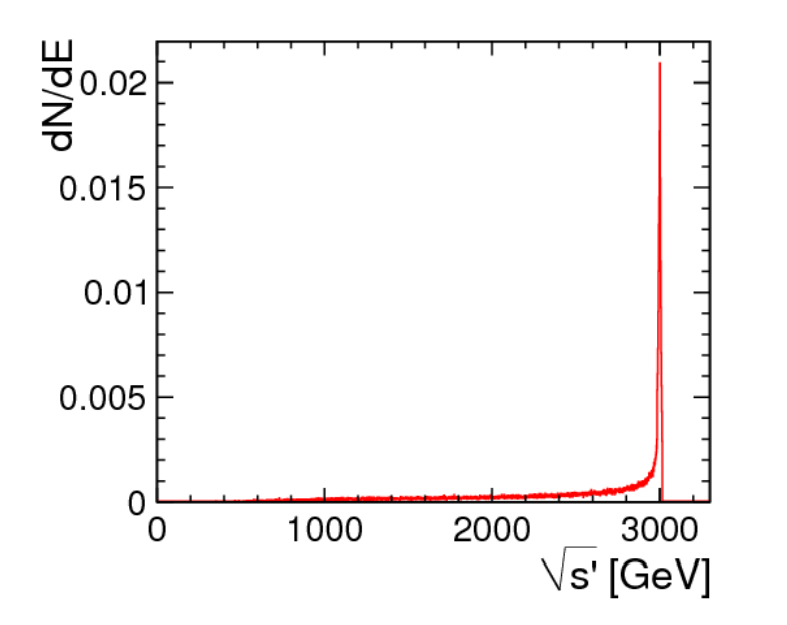
\includegraphics[width=0.7\linewidth]{{images/beamsstrahlung}.png}
  \caption{The luminosity spectrum for CLIC operating at $\surd s$ = 3 TeV, where $\surd s'$ is the
  effective centre-of-mass energy after beamstrahlung and initial state radiation }
  \label{fig2.15}
\end{figure}






\chapter{Supersymmetry}

\section{}

This section should be written in standard scientific
language. Standard techniques in your research field should not be
written out in detail. In computational projects this section should
be used to explain the algorithms used and the layout of the
computational code. A copy of the actual code may be given in the
appendices if appropriate.

This section should emphasise the philosophy of the approach used and
detail novel techniques. However please note: this section should not
be a blow-by-blow account of what you did throughout the project. It
should not contain large detailed sections about things you tried and
found to be completely wrong! However, if you find that a technique
that was expected to work failed, that is a valid result and should be
included.

Here logical structure is particularly important, and you may find
that to maintain good structure you may have to present the
explorations/calculations/computations/whatever in a different order
from the one in which you carried them out.


You might sometimes want to include multiple equations in one place
\begin{eqnarray}
  E &=& ma^{2} \\
  E &=& mb^{2} \\
  E &=& mc^{2}
\end{eqnarray}
You might want to include multiple equations in one place without
numbering them
\begin{eqnarray*}
  E &=& ma^{2} \\
  E &=& mb^{2} \\
  E &=& mc^{2}
\end{eqnarray*}
You might want to include multiple equations in one place without
numbering \emph{all} of them
\begin{eqnarray}
  E &=& ma^{2} \nonumber \\
  E &=& mb^{2} \nonumber \\
  E &=& mc^{2}
\end{eqnarray}

You might also want to include diagrams.  The example shows the use of
the special command which allows existing postscript files to be
included.  You would normally keep your figures separate from the text. 
These pictures might be images or pdf output from some
program.

Below I create a figure which is centred and stretched to 30\% of the
width of the page \verb+{0.30\hsize}+ and with the height stretched by
the same amount \verb+{!}+ to preserve the aspect ratio. If you omit
the extension (ie .eps, .ps or .pdf) on the file name then \LaTeX\ will
pick up the postscript copy whereas pdflatex will automatically pick
up the PDF version.


\begin{figure}

\begin{center}
  \resizebox{0.30\hsize}{!}{
\includegraphics{crest.pdf}}
\end{center}

\caption{The University Crest}
\label{fig:eucrest}

\end{figure}

You should find the file crest.pdf on this wiki.

% note that labels do not need to include a description of the object
% they are labelling but it can be helpful, eg \label{fig:figurename}.

You can use a label on a figure to refer to it later. The university
crest is in Figure~(\ref{fig:eucrest}). Note that you should not use
phrases like ``the figure above'' or ``the following figure'' since
\LaTeX\ may move the figure relative to the text if it cannot be fitted
onto the current page.

\chapter{Another Chapter Title}
\section{Number of Chapters}

You may vary the number of chapters. The Introduction and Background
Theory chapter are essential, although you may choose a different
title for the latter. These two introductory chapters are usually
followed by a chapter on what you did yourself, with a title such as
Design and Development, although you can choose any title you
wish. After that, you might to have another chapter, or you may go
straight to the Results and Conclusions chapter.

After the Introduction, you are free to use any chapter titles you wish.


\chapter{Results and Analysis}

This section should detail the obtained results in a clear,
easy-to-follow manner. It is important to make clear what are original
results and what are repeats of previous calculations or computations.
Remember that long tables of numbers are just as boring to read as
they are to type-in!

Use graphs to present your results wherever practicable.

Results or computations should be presented with uncertainties
(errors), both statistical and systematic where applicable.

Be selective in what you include: half a dozen \emph{e.g.}~tables that
contain wrong data you collected while you forgot to switch on the
computer are not relevant and may mask the correct results.


\section{Some results}
Here are some results.

\subsection{More results}
When showing results you are likely to use tables and graphs. You can
create tables easily in \LaTeX.

\begin{table}[h]
\begin{center}
\begin{tabular}{||l|c|l||}
\hline
\textbf{File names} & \textbf{Satellite} & \textbf{Resolution}\\
\hline
  worldr            &  Meteosat          &   5km\\
  worldg            &  Meteosat          &   5km\\
  worldb            &  Meteosat          &   5km\\
\hline
\end{tabular}
\end{center}
\caption{This is a simple table. More complicated tables can have
headings which pass over more than one column}
\label{simple_table}
\end{table}

If you want to produce fancier tables than shown in Table \ref{simple_table}
refer to the \LaTeX\ manual or ask Google.

One of the simplest ways to produce simple graphs is to use gnuplot
which produces \LaTeX\  output. Graph~(\ref{fig:gnu}) was produced using
gnuplot with output designated as \LaTeX\  so that a \LaTeX\  output file is
produced which you can include directly or keep separate and refer to
using the \emph{include} command.

Another approach is to draw simple figures using \emph{xfig} which allows
you to export diagrams in \LaTeX\  picture format so that the diagram can
be included directly.

Perhaps the most robust way to include graphs is to convert them to
PostScript or PDF and include them in the same was as was done in
Figure~\ref{fig:eucrest} for the University Crest. You can usually do
this with most packages, including Microsoft ones; one trick for
producing PostScript is to print to a dummy PostScript printer.

% in practice you would probably keep this in a separate file and use
% the \include{filename} command to insert it here.

\begin{figure}
% GNUPLOT: LaTeX picture
\setlength{\unitlength}{0.240900pt}
\ifx\plotpoint\undefined\newsavebox{\plotpoint}\fi
\sbox{\plotpoint}{\rule[-0.200pt]{0.400pt}{0.400pt}}%
\begin{picture}(1500,1200)(0,0)
\font\gnuplot=cmr10 at 10pt
\gnuplot
\sbox{\plotpoint}{\rule[-0.200pt]{0.400pt}{0.400pt}}%
\put(220.0,113.0){\rule[-0.200pt]{292.934pt}{0.400pt}}
\put(220.0,113.0){\rule[-0.200pt]{0.400pt}{245.477pt}}
\put(220.0,113.0){\rule[-0.200pt]{4.818pt}{0.400pt}}
\put(198,113){\makebox(0,0)[r]{$0$}}
\put(1416.0,113.0){\rule[-0.200pt]{4.818pt}{0.400pt}}
\put(220.0,317.0){\rule[-0.200pt]{4.818pt}{0.400pt}}
\put(198,317){\makebox(0,0)[r]{$0.2$}}
\put(1416.0,317.0){\rule[-0.200pt]{4.818pt}{0.400pt}}
\put(220.0,521.0){\rule[-0.200pt]{4.818pt}{0.400pt}}
\put(198,521){\makebox(0,0)[r]{$0.4$}}
\put(1416.0,521.0){\rule[-0.200pt]{4.818pt}{0.400pt}}
\put(220.0,724.0){\rule[-0.200pt]{4.818pt}{0.400pt}}
\put(198,724){\makebox(0,0)[r]{$0.6$}}
\put(1416.0,724.0){\rule[-0.200pt]{4.818pt}{0.400pt}}
\put(220.0,928.0){\rule[-0.200pt]{4.818pt}{0.400pt}}
\put(198,928){\makebox(0,0)[r]{$0.8$}}
\put(1416.0,928.0){\rule[-0.200pt]{4.818pt}{0.400pt}}
\put(220.0,1132.0){\rule[-0.200pt]{4.818pt}{0.400pt}}
\put(198,1132){\makebox(0,0)[r]{$1$}}
\put(1416.0,1132.0){\rule[-0.200pt]{4.818pt}{0.400pt}}
\put(220.0,113.0){\rule[-0.200pt]{0.400pt}{4.818pt}}
\put(220,68){\makebox(0,0){$0$}}
\put(220.0,1112.0){\rule[-0.200pt]{0.400pt}{4.818pt}}
\put(414.0,113.0){\rule[-0.200pt]{0.400pt}{4.818pt}}
\put(414,68){\makebox(0,0){$1$}}
\put(414.0,1112.0){\rule[-0.200pt]{0.400pt}{4.818pt}}
\put(607.0,113.0){\rule[-0.200pt]{0.400pt}{4.818pt}}
\put(607,68){\makebox(0,0){$2$}}
\put(607.0,1112.0){\rule[-0.200pt]{0.400pt}{4.818pt}}
\put(801.0,113.0){\rule[-0.200pt]{0.400pt}{4.818pt}}
\put(801,68){\makebox(0,0){$3$}}
\put(801.0,1112.0){\rule[-0.200pt]{0.400pt}{4.818pt}}
\put(995.0,113.0){\rule[-0.200pt]{0.400pt}{4.818pt}}
\put(995,68){\makebox(0,0){$4$}}
\put(995.0,1112.0){\rule[-0.200pt]{0.400pt}{4.818pt}}
\put(1188.0,113.0){\rule[-0.200pt]{0.400pt}{4.818pt}}
\put(1188,68){\makebox(0,0){$5$}}
\put(1188.0,1112.0){\rule[-0.200pt]{0.400pt}{4.818pt}}
\put(1382.0,113.0){\rule[-0.200pt]{0.400pt}{4.818pt}}
\put(1382,68){\makebox(0,0){$6$}}
\put(1382.0,1112.0){\rule[-0.200pt]{0.400pt}{4.818pt}}
\put(220.0,113.0){\rule[-0.200pt]{292.934pt}{0.400pt}}
\put(1436.0,113.0){\rule[-0.200pt]{0.400pt}{245.477pt}}
\put(220.0,1132.0){\rule[-0.200pt]{292.934pt}{0.400pt}}
\put(45,622){\makebox(0,0){\shortstack{This is\\the\\$y$ axis}}}
\put(828,23){\makebox(0,0){This is the $x$ axis}}
\put(828,1177){\makebox(0,0){This is a plot of $y=sin(x)$}}
\put(220.0,113.0){\rule[-0.200pt]{0.400pt}{245.477pt}}
\sbox{\plotpoint}{\rule[-0.500pt]{1.000pt}{1.000pt}}%
\put(1306,1067){\makebox(0,0)[r]{sin(x)}}
\multiput(1328,1067)(20.756,0.000){4}{\usebox{\plotpoint}}
\put(1394,1067){\usebox{\plotpoint}}
\put(220,113){\usebox{\plotpoint}}
\multiput(220,113)(3.768,20.411){4}{\usebox{\plotpoint}}
\multiput(232,178)(4.132,20.340){3}{\usebox{\plotpoint}}
\multiput(245,242)(3.825,20.400){3}{\usebox{\plotpoint}}
\multiput(257,306)(3.884,20.389){3}{\usebox{\plotpoint}}
\multiput(269,369)(3.944,20.377){3}{\usebox{\plotpoint}}
\multiput(281,431)(4.326,20.300){3}{\usebox{\plotpoint}}
\multiput(294,492)(4.137,20.339){3}{\usebox{\plotpoint}}
\multiput(306,551)(4.276,20.310){3}{\usebox{\plotpoint}}
\multiput(318,608)(4.693,20.218){3}{\usebox{\plotpoint}}
\multiput(331,664)(4.583,20.243){2}{\usebox{\plotpoint}}
\multiput(343,717)(4.754,20.204){3}{\usebox{\plotpoint}}
\multiput(355,768)(5.034,20.136){2}{\usebox{\plotpoint}}
\multiput(367,816)(5.760,19.940){2}{\usebox{\plotpoint}}
\multiput(380,861)(5.579,19.992){3}{\usebox{\plotpoint}}
\put(398.00,923.50){\usebox{\plotpoint}}
\multiput(404,943)(7.049,19.522){2}{\usebox{\plotpoint}}
\multiput(417,979)(7.288,19.434){2}{\usebox{\plotpoint}}
\put(433.18,1021.10){\usebox{\plotpoint}}
\multiput(441,1040)(8.982,18.712){2}{\usebox{\plotpoint}}
\put(460.41,1076.97){\usebox{\plotpoint}}
\put(471.84,1094.28){\usebox{\plotpoint}}
\put(484.84,1110.41){\usebox{\plotpoint}}
\put(500.42,1124.01){\usebox{\plotpoint}}
\multiput(503,1126)(19.159,7.983){0}{\usebox{\plotpoint}}
\put(519.48,1131.37){\usebox{\plotpoint}}
\multiput(527,1132)(20.136,-5.034){0}{\usebox{\plotpoint}}
\put(539.74,1128.60){\usebox{\plotpoint}}
\put(557.04,1117.38){\usebox{\plotpoint}}
\put(570.79,1101.95){\usebox{\plotpoint}}
\put(582.44,1084.80){\usebox{\plotpoint}}
\put(593.09,1066.99){\usebox{\plotpoint}}
\multiput(601,1053)(8.430,-18.967){2}{\usebox{\plotpoint}}
\put(619.18,1010.54){\usebox{\plotpoint}}
\multiput(625,996)(7.413,-19.387){2}{\usebox{\plotpoint}}
\multiput(638,962)(6.403,-19.743){2}{\usebox{\plotpoint}}
\multiput(650,925)(5.830,-19.920){2}{\usebox{\plotpoint}}
\multiput(662,884)(5.461,-20.024){2}{\usebox{\plotpoint}}
\multiput(674,840)(5.533,-20.004){2}{\usebox{\plotpoint}}
\multiput(687,793)(4.937,-20.160){3}{\usebox{\plotpoint}}
\multiput(699,744)(4.667,-20.224){2}{\usebox{\plotpoint}}
\multiput(711,692)(4.858,-20.179){3}{\usebox{\plotpoint}}
\multiput(724,638)(4.276,-20.310){3}{\usebox{\plotpoint}}
\multiput(736,581)(4.205,-20.325){3}{\usebox{\plotpoint}}
\multiput(748,523)(4.070,-20.352){3}{\usebox{\plotpoint}}
\multiput(760,463)(4.326,-20.300){3}{\usebox{\plotpoint}}
\multiput(773,402)(3.884,-20.389){3}{\usebox{\plotpoint}}
\multiput(785,339)(3.884,-20.389){3}{\usebox{\plotpoint}}
\multiput(797,276)(4.070,-20.352){3}{\usebox{\plotpoint}}
\multiput(810,211)(3.825,-20.400){3}{\usebox{\plotpoint}}
\multiput(822,147)(3.607,-20.440){2}{\usebox{\plotpoint}}
\put(828,113){\usebox{\plotpoint}}
\end{picture}
\caption{Simple Gnuplot example}
\label{fig:gnu}
\end{figure}

\section{Discussion of your results}

This section should give a picture of what you have taken out of your
project and how you can put it into context.

This section should summarise the results obtained, detail conclusions
reached, suggest future work, and changes that you would make if you
repeated the project.

\chapter{Conclusions}

This is the place to put your conclusions about your work. You can
split it into different sections if appropriate. You may want to include
a section of future work which could be carried out to continue your
research.

The conclusion section should be at least one page long, preferably 2
pages, but not much longer.

\appendix
% the appendix command just changes heading styles for appendices.

\chapter{Stuff that's too detailed}

Appendices should contain all the material which is considered too
detailed to be included in the main body of the text, but which is
important enough to be included in the thesis.

Perhaps this is a good place to mention \BibTeX.

You can do references in the simple way explained in the introduction,
or you can use \BibTeX.


\section{\BibTeX}
\label{sec:bibtex}

It is convenient to use \BibTeX\ to compile your bibliography.  First
you need to create a .bib file e.g.  you may call it ref.bib Then you
can put all your references into the file with entries such as
\begin{verbatim}
@Book{ob:bornwolf,
     author = "Born, M and Wolf, E",
     title  = "Principles of Optics",
     publisher = "Cambridge University Press",
     year = 1999,
     edition = {7th},
}

@Article{jr:ashkin,
Author = {A. Ashkin and J.M. Dziedzic and J.E. Bjorkholm and S. Chu},
Title = "Observation of a single beam gradient force optical tap for 
dielectric particles",
Journal = "Optics Letters",
Volume = 11,
Pages = "288-290",
Year = 1986}

@INPROCEEDINGS{seger,
 author = {J. Seger and H.J. Brockman},
 title = {What is bet-hedging?},
 editors={P.H. Harvey and L. Partridge},
 booktitle = {Oxford Surveys in Evolutionary Biology},
 year={1987},
 page={18},
 publisher={Oxford University Press},
 place={Oxford}}
\end{verbatim}
for a book, an article in a journal or an article in a proceedings volume
respectively.

Inside your \LaTeX\ file
you should include 
\begin{verbatim}
\bibliographystyle{unsrt}                      
and
\bibliography{ref}
\end{verbatim}
The first command determines the reference style, here plain and 
unsorted. With this referencing style 
a numerical referencing system (which is now the most
common in physics literature) is used and the numbering of references
will be the order in which they appear in the document. Alternatively, 
you could use
a customised `style file' but there is no real need.  The second
command just inputs your .bib file Note that only the references cited
in the text will appear in the bibliography so you can have spare
references in your .bib file.


You use the name you have given to an entry (e.g.
for the book example above the name is ob:bornwolf)
to cite the relevant article
by using the cite command in your \LaTeX\ file e.g. \cite{ob:bornwolf}



\section{Producing your documents using \texttt{pdflatex}}

To use pdflatex your figures need to be in pdf format.  You can convert almost any image file to pdf using \texttt{convert}.  e.g. \texttt{convert myfigure.png myfigure.pdf}.

The first time you should type:
\begin{verbatim}
  pdflatex ProjectReport
  bibtex ProjectReport
  pdflatex ProjectReport
  pdflatex ProjectReport
\end{verbatim} 
This first time you run\texttt{pdflatex} it will produce a
\texttt{ProjectReport.aux}.  The \BibTeX\ command reads in the
bibliography file and makes the files \texttt{ProjectReport.bbl} and
\texttt{ProjectReport.blg} files.  These files are read in the next
\texttt{pdflatex} command, but you'll still have ``undefined
cross-reference'' errors which are sorted out by the last
\texttt{pdflatex} command.

Subsequently, you should only need to do one (or two)
\texttt{pdflatex}s, or \texttt{pdfbibtex} followed by
\texttt{pdflatex} twice if you change any references.

\vspace{5mm} You may also use plain \texttt{latex} instead of
\texttt{pdflatex}.  This requires you to use postscript graphics
instead of pdf.




\chapter{Stuff that won't be read by anyone}

Some people include in their thesis a lot of detail, particularly lots
of tables containing raw results, figures of intermediate results, or
computer code which no-one will ever read. You should be careful that
anything like this you include should contain some element of
uniqueness which justifies its inclusion.


\newpage

\bibliographystyle{unsrt}
\bibliography{MSc_dissertation}


\end{document}

